% -*-cap2.tex-*-
% Este fichero es parte de la plantilla LaTeX para
% la realización de Proyectos Final de Carrera, protegido
% bajo los términos de la licencia GFDL.
% Para más información, la licencia completa viene incluida en el
% fichero fdl-1.3.tex

% Copyright (C) 2009 Pablo Recio Quijano 

Para el desarrollo de \textbf{Dominous} se decidió utilizar el modelo evolutivo iterativo incremental para el ciclo de
vida del proyecto. La decisión fue tomada ya que, a pesar de tener acotado el ámbito y los requisitos del programa,
la funcionalidad concreta de cada uno de los apartados se desconocía en un principio.\\

El modelo iterativo incremental es un modelo de tipo evolutivo que está basado en varios ciclos en cascada realimentados aplicados
repetidamente, con una filosofía iterativa. Como se comenta en~\cite{ingenieriaIan}, al final de cada iteración se le
realiza una entrega al cliente final; en este caso, los clientes han sido los tutores del proyecto, que a cada iteración iban
dictando las líneas maestras generales a tomar a cada nuevo paso.\\

Las ventajas de utilizar un modelo iterativo incremental son básicamente los siguientes:
\begin{enumerate}
    \item Construir un sistema pequeño es siempre menos costoso en términos de riesgo.
    \item Al ir desarrollando parte de las funcionalidades, es más fácil determinar si los requisitos
            planeados para los niveles subsiguientes son correctos.
    \item Si se comete algún error grave, sólo la última iteración necesita ser descartada.
    \item Reduciendo el tiempo de desarrollo de un sistema (en este caso en incremento del sistema) decrecen las
            probabilidades que esos requerimientos de usuarios puedan cambiar durante el desarrollo.
    \item Los errores de desarrollo realizados en un incremento, pueden ser arreglados antes del comienzo del próximo incremento.
\end{enumerate}

El proyecto \textbf{Dominous} consta de tres subsistemas que son los que ocupan el grueso del desarrollo:
\begin{enumerate}
    \item El primero es el motor de la partida: Controla los jugadores, las fichas en la mesa, la partida, situaciones irregulares
            y cualquier otro elemento referente únicamente al ámbito del dominó.
    \item Por otro lado está el motor gráfico, que será la interfaz entre la partida y el usuario, permitiendo el movimiento
            fluido por las diferentes secciones del programa e interactuando de forma directa con el motor de la partida,
            mostrando las fichas actuales y habilitando la interacción del jugador con el mundo.
    \item Y por último tenemos el motor de Inteligencia Artificial. Este motor será el que alimente la inteligencia
            y las acciones y decisiones de los jugadores controlados por el ordenador.
\end{enumerate}

\section{Organización de las partes básicas de la aplicación}

Después de analizar minuciosamente los requisitos de la aplicación, se decidió atacar al grueso de la misma,
es decir, la gestión de una partida de dominó en sí, y se estimó que esta debería dividirse en los siguientes
apartados:

\begin{description}
    \item[Subsistema de gestión de la partida] Este subsistema se encarga de gestionar todo lo relacionado
            con el control de la partida que se desarrolla actualmente. Desde el conteo de puntos por parte
            de cada equipo hasta las fichas de cada jugador, pasando por comprobaciones de que la partida
            se desarrolla con normalidad y no se producen violaciones de las reglas y normas, barajar las
            fichas, comprobar que se cierra la partida o pedir fichas a los diferentes jugadores.
    \item[Subsistema gráfico] Su labor es mostrar por pantalla la información que controla el subsistema
            de gestión de la partida. Debe dibujar en la pantalla el tablero con las fichas colocadas
            actualmente, las fichas de cada jugador, los puntos de cada equipo y demás información que
            sea necesario mostrar.
    \item[Subsistema de Inteligencia Artificial] Este último apartado se encarga de dotar de inteligencia al
            conjunto de jugadores que intervienen en la partida y que están controlados por el ordenador. Incluye
            crear los sistemas expertos, las bases de conocimiento, la librería de reglas y las diferentes
            interfaces entre el juego y el sistema de gestión de la partida.
\end{description}

Una vez dividido todo el proyecto en módulos podemos realizar una estimación de tiempos a partir del cual se
obtiene el diagrama de Gantt~\ref{fig:diag_gantt}.

\begin{itemize}
    \item Toma de requisitos --- 27d
        \begin{itemize}
            \item Requisitos de hardware --- 1d
            \item Requisitos de software --- 16d
            \item Comprobación de requisitos --- 9d
        \end{itemize}
    \item Investigación preliminar --- 80d
        \begin{itemize}
            \item Análisis del estado del arte --- 5d
            \item Bibliotecas de desarrollo --- 75d
        \end{itemize}
    \item Planificación --- 27d
    \item Análisis del sistema --- 28d
    \item Diseño del sistema --- 265d
    \item Implementación --- 236d
        \begin{itemize}
            \item Subsistema de gestión de partida --- 130d
            \item Subsistema de Inteligencia Artificial --- 140d
            \item Subsistema gráfico --- 80d
        \end{itemize}
    \item Pruebas --- 20d
        \begin{itemize}
            \item Pruebas unitarias ---16d
            \item Pruebas de integración --- 1d
            \item Pruebas de jugabilidad y experiencia de usuario ---3d
        \end{itemize}
    \item Redacción de la memoria --- 62d
\end{itemize}

\begin{figure}[h]
  \begin{center}
    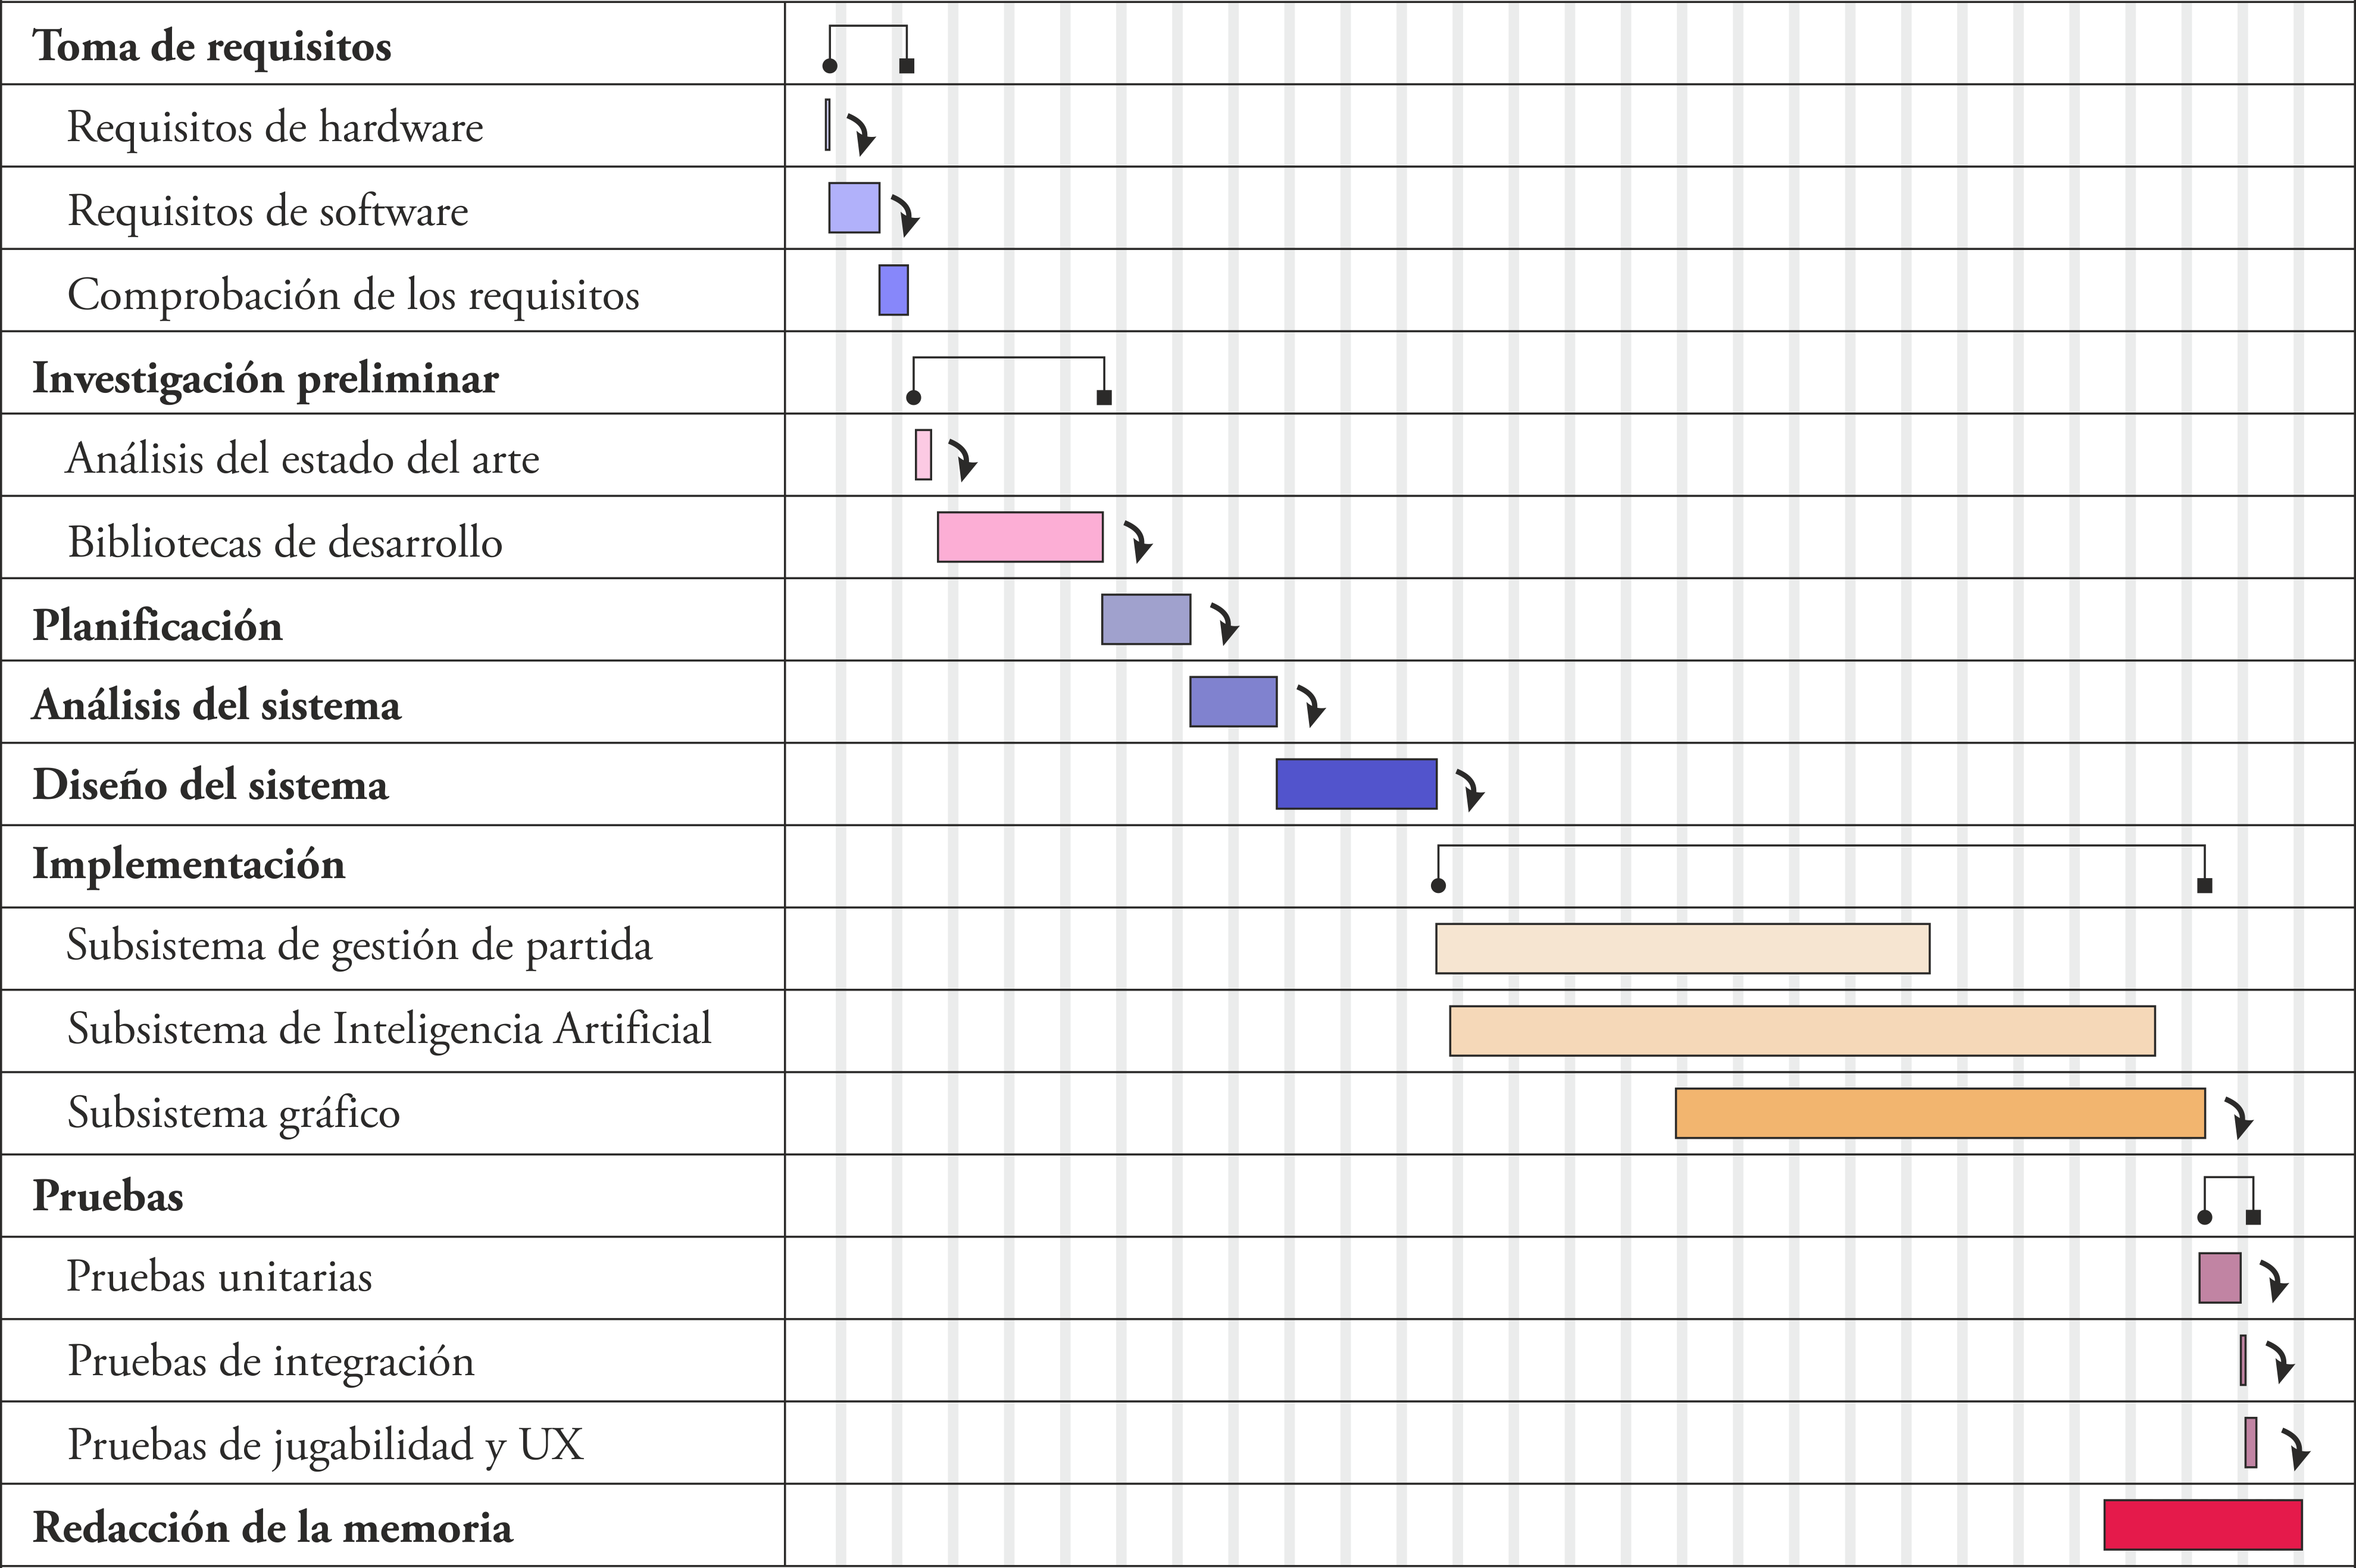
\includegraphics[angle=90,scale=0.60]{diagrama_gantt.png}
  \end{center}
  \caption{Diagrama de Gantt}
  \label{fig:diag_gantt}
\end{figure}
